% !TEX TS-program = pdflatex
% !TEX encoding = UTF-8 Unicode

% This is a simple template for a LaTeX document using the "article" class.
% See "book", "report", "letter" for other types of document.

\documentclass{article} 
\usepackage[14pt]{extsizes} %задаем размер шрифта

\usepackage[utf8]{inputenc} % set input encoding (not needed with XeLaTeX)
\usepackage[T2A]{fontenc}
\usepackage[pages=some]{background}
\usepackage{graphicx} % support the \includegraphics command and options
\usepackage[most]{tcolorbox} % для управления цветом

\definecolor{sw}{RGB}{229,177,58} %Цвет текста звездных войн эпизода 1
\definecolor{sky_black}{RGB}{17,16,10} %Цвет ночного неба
% Настройка для рамки вокруг текста
\definecolor{block-gray}{gray}{0.90} % уровень прозрачности (1 - максимум)
\newtcolorbox{myquote}{colframe=sw, colback=black,grow to right by=-10mm,grow to left by=-10mm,
boxrule=2pt,boxsep=0pt} % настройки области с изменённым фоном

\backgroundsetup{
scale=1,
color=black,
opacity=1,
angle=0,
contents={%
  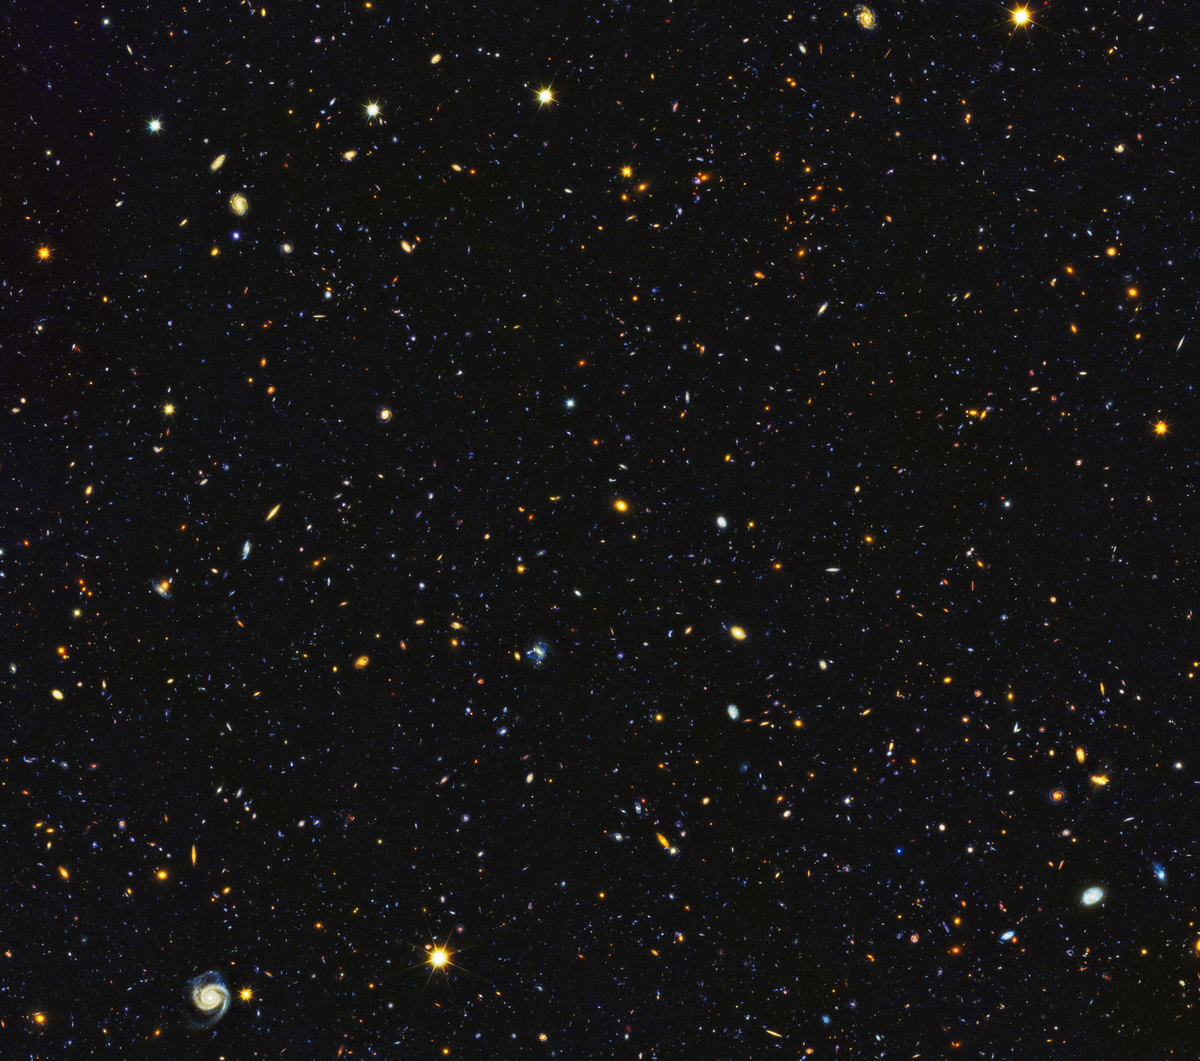
\includegraphics[width=\paperwidth,height=\paperheight]{imgs/stars_img.jpg}
  }%
}

\title{Забытый артефакт}
\author{SW Duncan's community}
%\date{} % Activate to display a give date or no date (if empty),
         % otherwise the current date is printed 

\color{sw}
\begin{document}
\pagecolor{sky_black}
\BgThispage
\maketitle %титульная страница
\newpage
\tableofcontents %оглавление
\newpage
\section{В поисках храма}

\begin{myquote}
%\pagecolor{black}
\color{sw}
\input{envs/planet.tex}
\end{myquote}
\subsection{Воздушный вояж}
\begin{myquote}
\color{sw}
\input{envs/fly_good.tex}
\end{myquote}


\begin{myquote}
\color{sw}
\input{envs/fly_bad.tex}
\end{myquote}
\subsection{С дипломатической миссией к каннибалам}
\begin{myquote}
\color{sw}
\input{envs/landing.tex}
\end{myquote}

\begin{myquote}
\color{sw}
\input{envs/village_far.tex}
\end{myquote}

\begin{myquote}
\color{sw}
\input{envs/village_to_temple.tex}
\end{myquote}

\section{Храм лорда ситхов}

\begin{myquote}
\color{sw}
\input{envs/temple.tex}
\end{myquote}

\begin{myquote}
\color{sw}
Бродя по храму, вы наткнулись на комнату, полную злобных духов, возвращенных к жизни могучим ситхским лордом.
Пол комнаты покрыт застарелой кровью - явный признак темных ритуалов. Вероятно, описание самих ритуалов можно найти тут же, все стены комнаты исписаны странными символами, которые вы видели ранее.
Ваши шаги гулко раздаются по всему помещению, поэтому скрыться вряд ли получится.
Впереди видна массивная запертая дверь, за которой явно скрывается главная гробница. К сожалению, призраки не настроены вас туда пропустить.

\end{myquote}
Призракам не нанести урон бластерами или световыми мечами.
Бороться с ними придется на ментальном фронте, объединив усилия и создавая Волны тьмы, отправляющие призраков назад в Бездну.
Кроме того, вам может помочь Светлый дух, вызвав Стену света (если, конечно, вам не противно применение Светлой стороны в своем присутствии)
Если подпустить призрака слишком близко к себе, он сможет овладеть вашим разумом и свести с ума, так что будьте осторожны и следите за своими товарищами - любой из них может вонзить меч вам в спину.
\end{document}
